\documentclass[12pt]{article}
\usepackage[T2A]{fontenc}
\usepackage[utf8]{inputenc}
\usepackage{multirow}
\usepackage{caption}
\usepackage{subcaption}
\usepackage{amsmath}
\usepackage{changepage}
\usepackage{graphicx}
\usepackage{float}
\usepackage[english,russian]{babel}
\usepackage{amsmath, amsfonts, amssymb, amsthm, mathtools}
\usepackage{xcolor}
\usepackage{array}
\usepackage{hyperref}
\usepackage{icomma}
\usepackage{mathtext} 
\usepackage[top = 1.5cm, left = 1.5 cm, right = 1.5 cm, bottom = 3 cm]{geometry}
\graphicspath{ {./images/} }
 
\title{Колебания в электрических цепях}
\author{Шахматов Андрей, Б02-304}
\date{\today}
  
\begin{document}
\begin{titlepage}
	\begin{center}
		{\large МОСКОВСКИЙ ФИЗИКО-ТЕХНИЧЕСКИЙ ИНСТИТУТ (НАЦИОНАЛЬНЫЙ ИССЛЕДОВАТЕЛЬСКИЙ УНИВЕРСИТЕТ)}
	\end{center}
	\begin{center}
		{\large Физтех-школа физики и исследований им. Ландау}
	\end{center}

	\vspace{3cm}
	{\huge
		\begin{center}
			\textbf{Колебания в электрических цепях}
		\end{center}
	}
	\vspace{2cm}
	\begin{flushright}
		{\LARGE Автор:\\ Шахматов Андрей Юрьевич \\
			\vspace{0.2cm}
			Б02-304}
	\end{flushright}
	\vspace{7 cm}
	\begin{center}
		Долгопрудный 2024
	\end{center}
	\thispagestyle{empty}
\end{titlepage}

% \maketitle

\begin{abstract}
	Исследовано изменение периода колебаний колебательного RLC контура от его ёмкости. Исследовано 
	изменение добротности контура при изменении его сопротивления. Изучен вид затухающих колебаний на фазовой 
	диаграмме. Рассмотрен процесс установления колебаний в контуре. 
\end{abstract}

% \tableofcontents

\section*{Введение}
Цель работы заключается в исследование характеристик колебательного контура, состоящего из катушки индуктивности, конденсатора и 
сопротивления.

\section*{Методика}
\subsection*{Уравнение колебаний в последовательном контуре}
Запишем равенство ЭДС в контуре относительно заряда:
\begin{equation}
	L\ddot{q} + R \dot{q} + \frac{q}{C} = \varepsilon(t),
\end{equation}
где $L$ --- индуктивность катушки, $R$ --- сопротивление резистора, $C$ --- ёмкость контенсатора.
Поделим на $L$ и введём новые обозначения:
\[
	\ddot{q} + 2\gamma \dot{q} + \omega_0^2 q = \frac{\varepsilon(t)}{L},
\]
где $\gamma = \frac{R}{2L}$ --- коэффициент затухания, $\omega_0 = \sqrt{\frac{1}{LC}}$ --- собственная частота контура.
Решение такого уравнения представляется в виде суммы частного решения общего решения уравнения:
\[
	\ddot{q} + 2\gamma \dot{q} + \omega_0^2 q = 0.
\]
Запишем характеристическое уравнение:
\[
	\lambda^2 + 2\gamma \lambda + \omega_0^2 = 0.
\]
Это обыкновенное квадратное уравнение имеет. Запишем его дискриминант:
\[
	\frac{D}{4} = \gamma^2 - \omega^2
\]
Общее решение имеет вид $\lambda = -\gamma \pm \sqrt{\gamma^2 - \omega^2}$
Тогда возможны 3 случая: $\gamma > \omega$, $\gamma = \omega$, $\gamma < \omega$.
В первом случае дискриминант положителен, во втором случае уравнение имеет два совпадающий решения,
в третьем случае уравнение имеет два комплексных решения. Можно ввести дополнительную величину
\begin{equation}
	R_{\text{кр}} = 2\sqrt{\frac{L}{C}} > R > 0,
\end{equation}
называемая волновым сопротивлением контура.
Тогда общее решение для первого и третьего случая имеет вид:
\begin{equation}
	q = Ae^{\left( -\gamma + \sqrt{\gamma^2 - \omega^2} \right) t } + Be^{\left( -\gamma - \sqrt{\gamma^2 - \omega^2} \right) t }.
\end{equation}
В первом случае уравнение останется в таком виде, тогда заряд будет экспоненциально уменьшаться до нуля,
колебаний не произойдёт.
Во третьем случае комплексные экспоненты преобразуются в синусы и косинусы по формуле Эйлера(при этом
комплексные части сократятся), тогда
решение можно переписать в виде:
\begin{equation}
	q = q_0 e^{-\gamma t} \cos(\sqrt{\omega^2 - \gamma^2}t + \varphi_0) = q_0 e^{-\gamma t} \cos(w_1 t + \varphi_0).
\end{equation}
Такой режим представляет затухающие колебания.
Во втором же случае решение представляет собой
\begin{equation}
	q = A t e^{\gamma t} + B e^{\gamma t}.
\end{equation}
Такой режим также представляет экспоненциально затухающее апериодическое поведение.
После этого достаточно найти частное решение исходного уравнения и сложить с общим. Аналогичное уравнение может
быть получено для $U$ на конденсаторе делением полученного уравнения на $C$.
\subsection*{Установление колебаний}
Рассмотрим внешнее ЭДС изменяющееся по закону:
\[
	\varepsilon = \varepsilon_0 \sin \omega t.
\]
Согласно предыдущему разделу общее решение представляется в виде:
\[
	U = U_0 e^{-\gamma t} \cos (w_1 t + \varphi_0) + A \cos (wt + \psi).
\]
Примем в качестве начальных условий $U = 0$, $\dot{U} = 0$ и преобразуем уравнение:
\[
	U = A \left( \sin (wt + \psi) - e^{-\gamma t} \sin (w_1 t + \psi) \right)
\]
В случае сильного отличия $w_1$ от $w$ будут наблюдаться биения, однако при небольшом отличие и высокой
добротности контура уравнение установления колебаний будет иметь вид:
\begin{equation}
	U = Q \varepsilon_0 \left( 1 - e^{-\gamma t} \right) \sin \omega_0 t,
\end{equation}
где $Q$ - добротность контура.


\subsection*{Описание установки}
\begin{figure}[H]
	\centering
	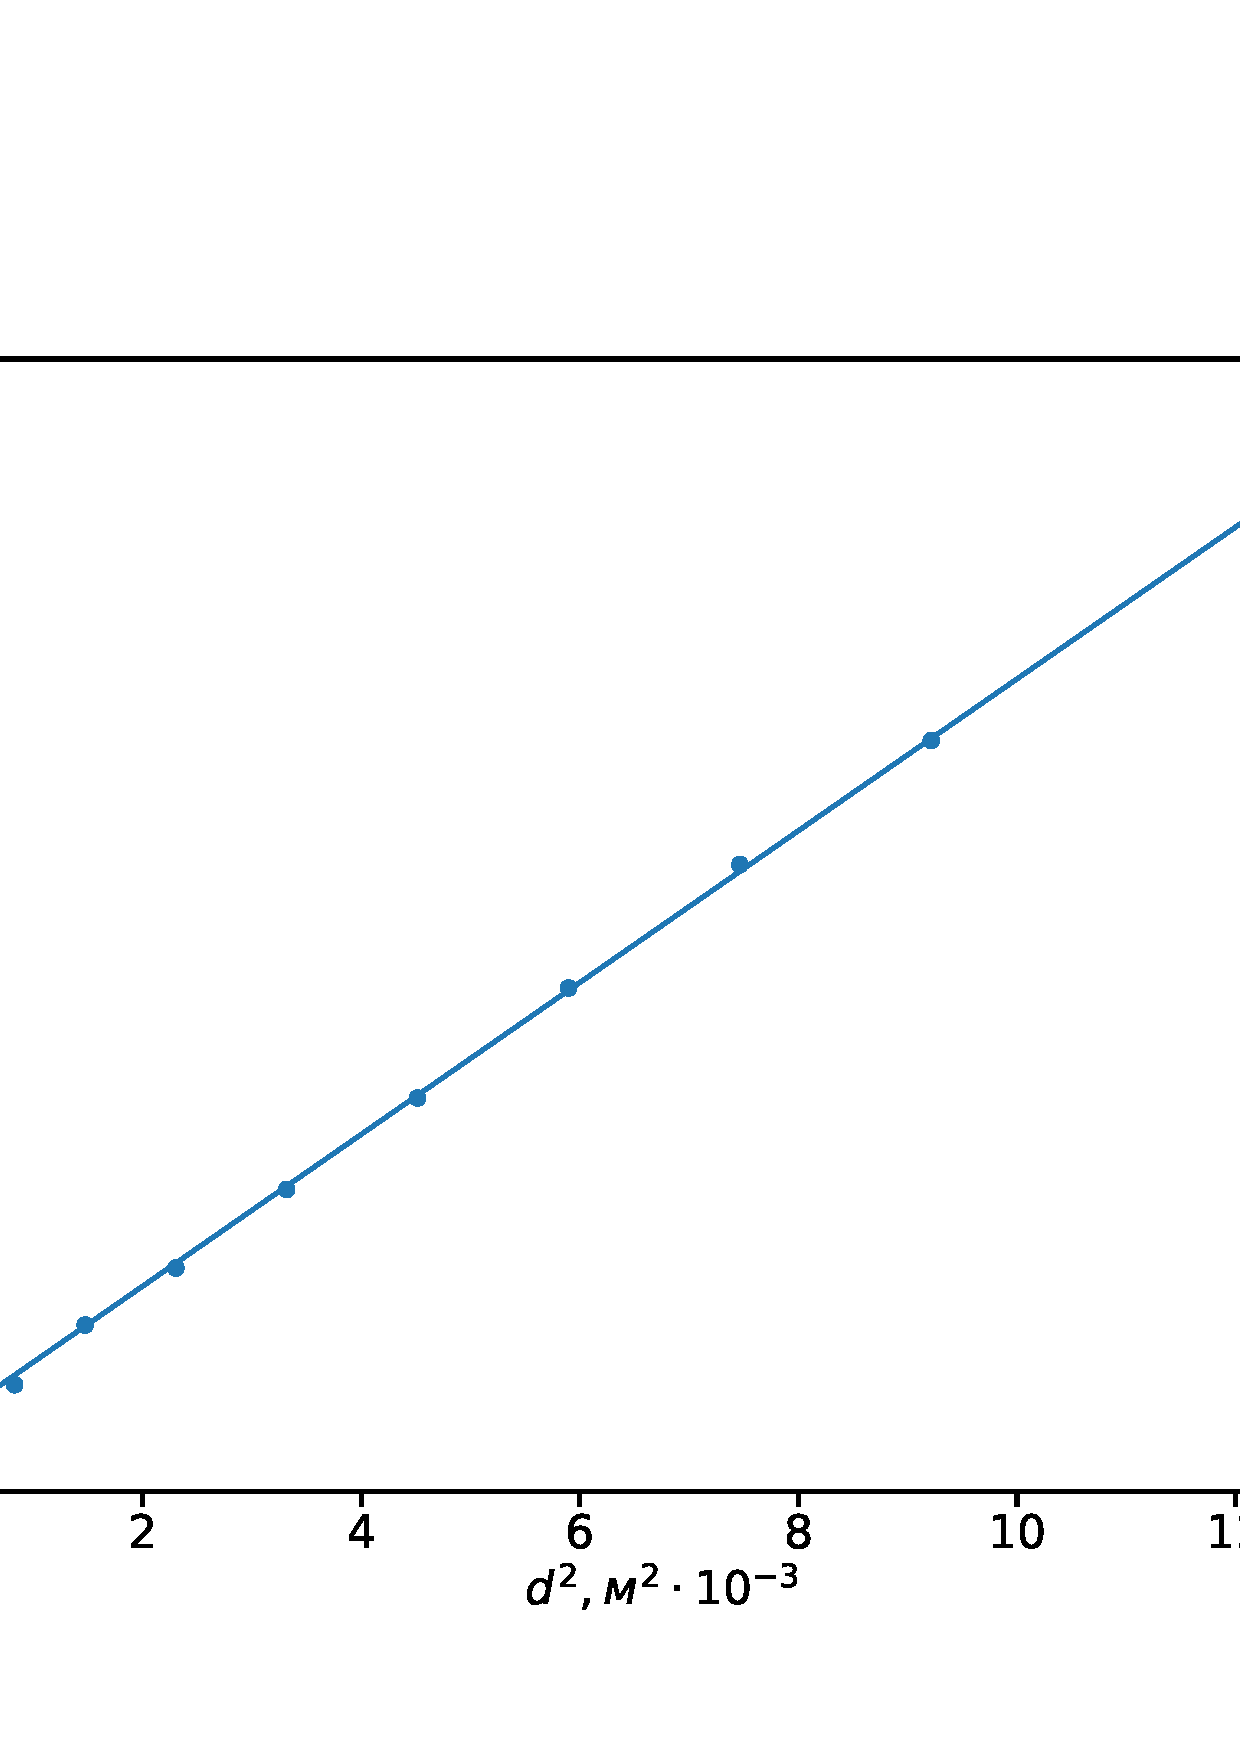
\includegraphics[width=0.7\textwidth]{1.png}
	\caption{Схема установки}
	\label{pic:scheme}
\end{figure}
На рисунке приведена схема для исследования свободных колебаний в контуре, содержащем постоянную индуктивность $L$ и переменные ёмкость $C$ и сопротивление $R$. Колебания наблюдаются на экране осциллографа.

Для периодического возбуждения колебаний в контуре используется генератор импульсов Г5-54. С выхода генератора по коаксиальному кабелю импульсы поступают на колебательный контур через электронное реле, смонтированное в отдельном блоке (или на выходе генератора). Реле содержит тиристор $D$ и ограничительный резистор $R_1$.
Импульсы заряжают конденсатор $C$. После каждого импульса генератор отключается от колебательного контура, и в контуре возникают свободные затухающие колебания. Входное сопротивление осциллографа велико ($\approx 1$ МОм), так что его влиянием на контур можно пренебречь. Для получения устойчивой картины затухающих колебаний используется режим ждущей развёртки с синхронизацией внешними импульсами, поступающими с выхода <<синхроимпульсы>> генератора.

\section*{Результаты и их обсуждение}
При нулевой ёмкости на конденсаторе измерен период затухающих колебаний.
По полученным данным найдена ёмкость контура, которая составила $\Delta C \approx 1 \text{ нФ}$.
Далее катушке выставлена индуктивность $L = 0,1 \text{ Гн}$.
Для первого опыта выставлено сопротивление $R = 410 \text{ Ом}$. Измерена зависимость периода колебаний от ёмкости конденсатора (Таблица \ref{tab:1}).
\begin{table}[H]
	\centering
	\begin{tabular}{|r|r|}
		\hline
		$C$, мкФ & $T$, мкс \\ \hline
		0        & 65       \\ \hline
		0,001    & 91       \\ \hline
		0,002    & 111      \\ \hline
		0,003    & 127      \\ \hline
		0,004    & 142      \\ \hline
		0,005    & 155      \\ \hline
		0,006    & 168      \\ \hline
		0,007    & 179      \\ \hline
		0,008    & 190      \\ \hline
		0,009    & 200      \\ \hline
	\end{tabular}
	\caption{Данные измерения зависимости периода затухающий колебаний $T$ от ёмкости конденсатора $C$.}
	\label{tab:1}
\end{table}
По полученным данным построен график зависимости периода колебаний от ёмкости конденсатора (Рис. \ref{fig:CT}). На основании теоретической
зависимости $T = 2 \pi \sqrt{LC} $ построена сглаживающая кривая. Видно, что кривая не выходит из точки $(0, 0)$, а сдвинута на ёмкость контура $\Delta C$.

\begin{figure}[H]
	\centering
	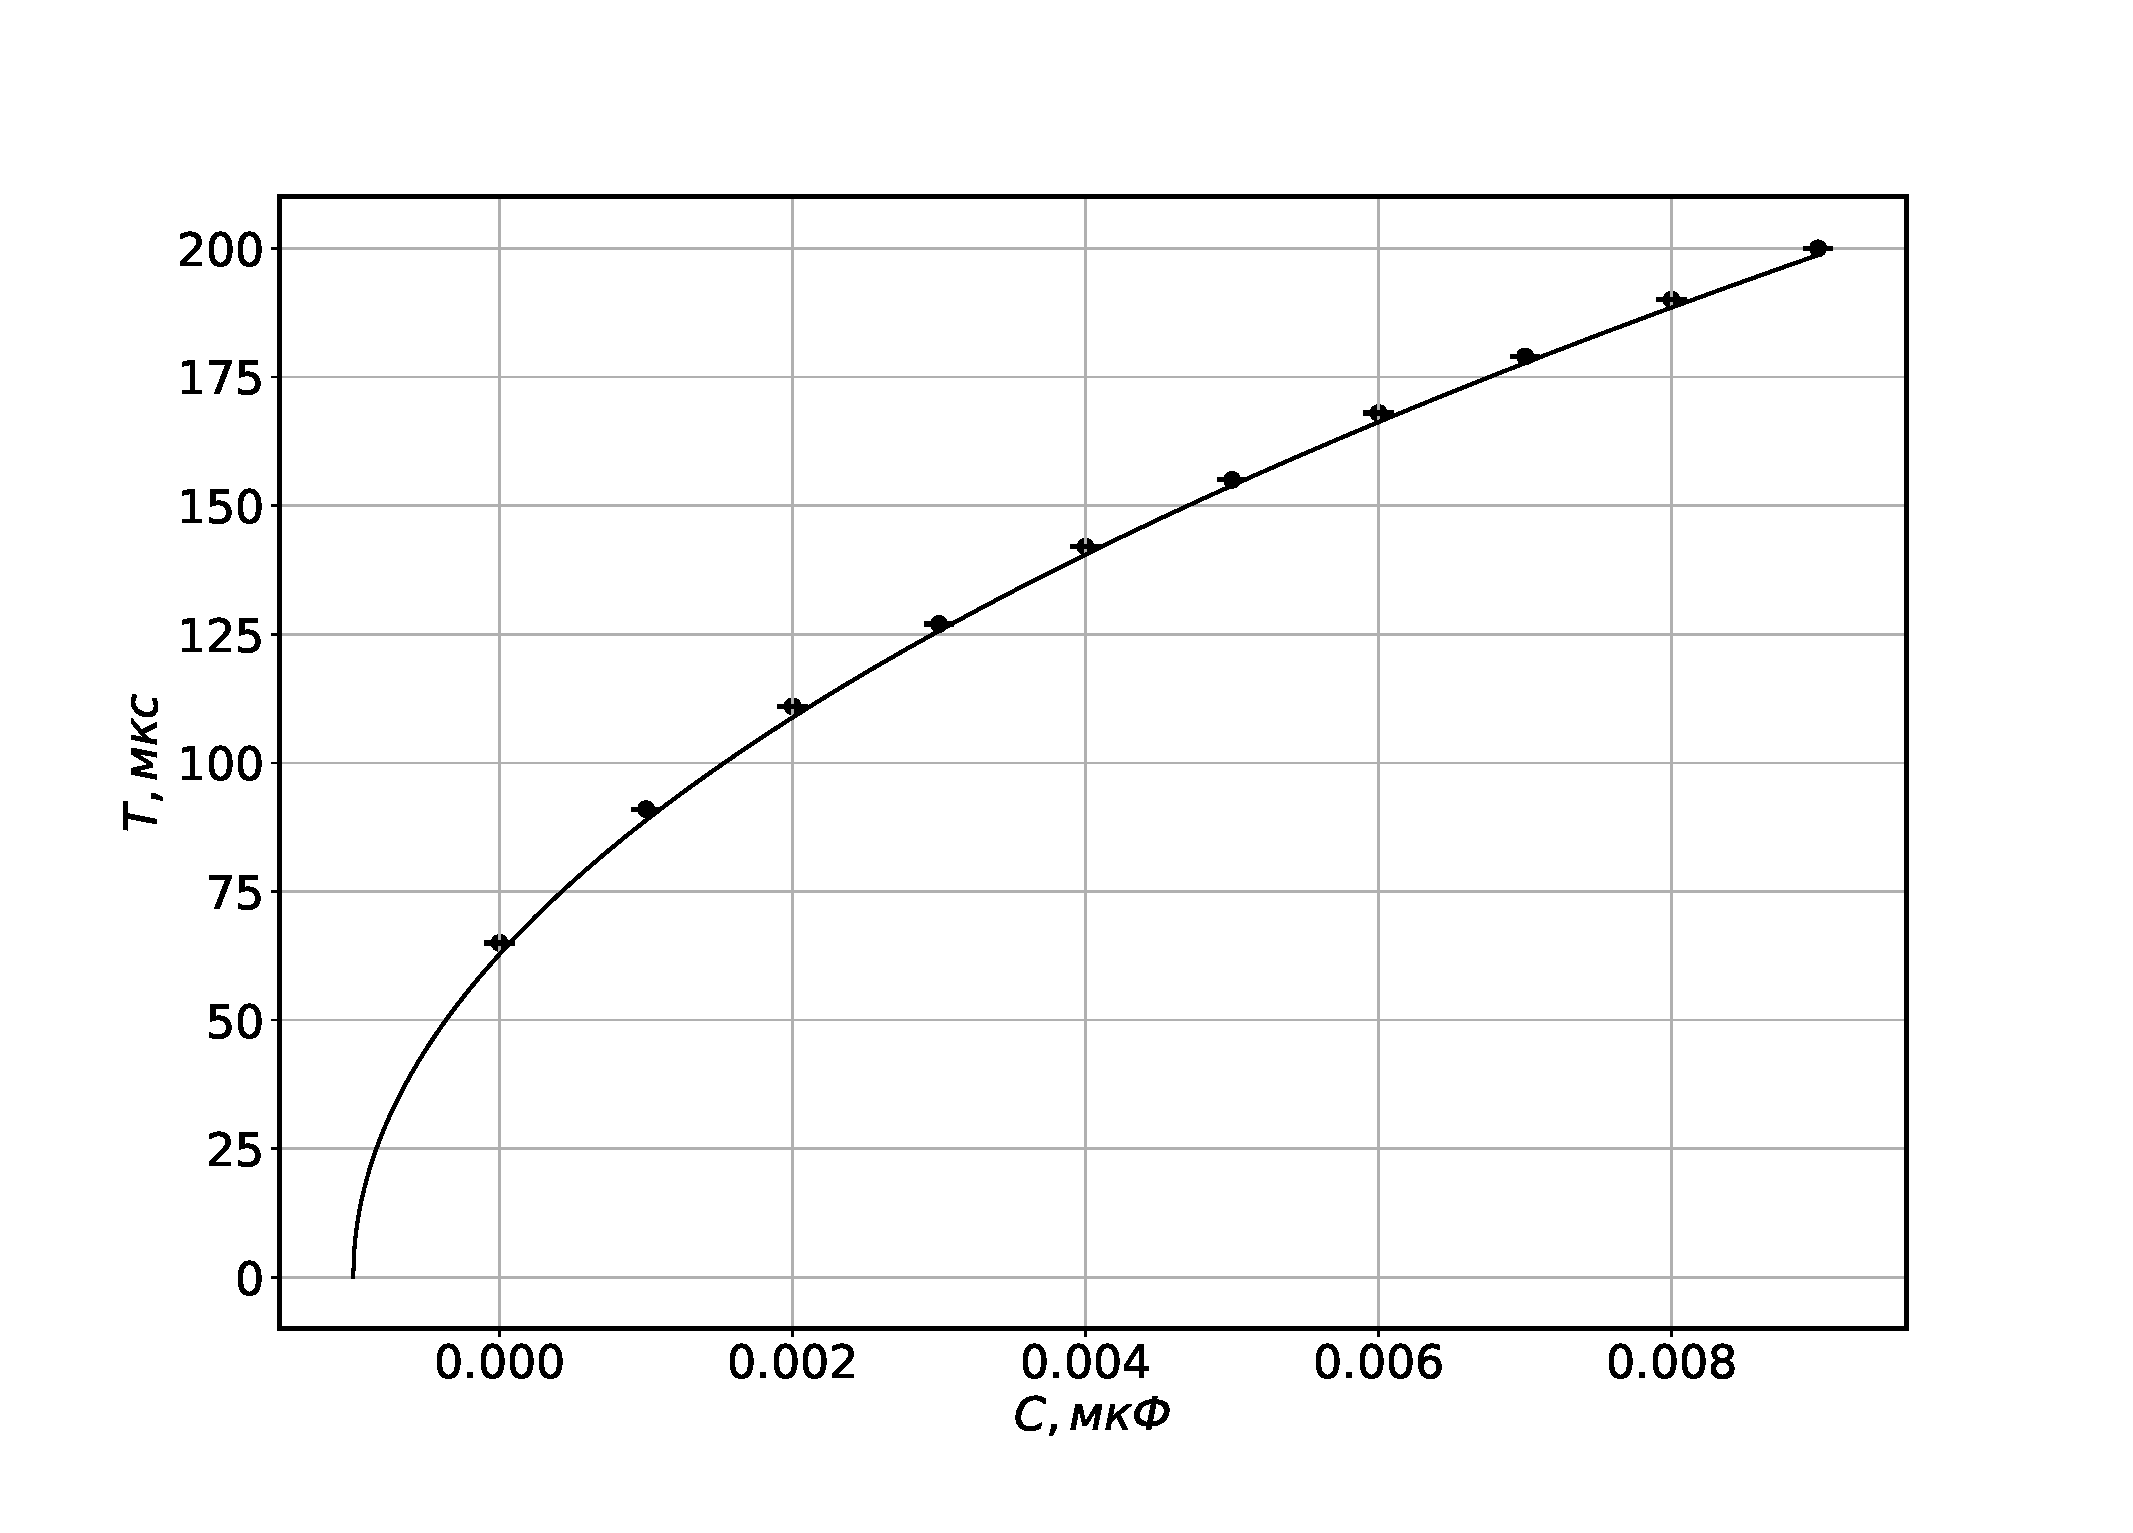
\includegraphics[width=0.7\textwidth]{CT.eps}
	\caption{График зависимости периода колебаний контура $T$ от ёмкости конденсатора $C$.}
	\label{fig:CT}
\end{figure}

Значения индуктивности катушки $L$ и ёмкости конденсатора $C$ установлены на $0,1 \text{ Гн}$ и $5 + 1 \text{ мкФ}$ соответственно, 
критическое сопротивление конутра при таких параметрах можно рассчитать как $R_{\text{кр}} = 2\pi \sqrt{\frac{L}{C}} = 8,1 \pm 0,1$ кОм. 
Измерены значения амплитуд затухающий колебаний в нескольких точках и на основе формулы
\[
	\theta = \frac{1}{k} \ln \frac{U_n}{U_{n + k}}
\]
рассчитаны декременты затухания и добротность контура (Таблица \ref{tab:2}).
\begin{table}[H]
	\centering
	\begin{tabular}{|r|r|r|r|r|r|}
		\hline
		k & $R$ , Ом & $U_1$, В & $U_2$, В & $\theta$ & $Q$  \\ \hline
		4 & 410      & 2,22     & 0,54     & 0,35     & 8,89 \\ \hline
		4 & 810      & 2,59     & 0,17     & 0,68     & 4,61 \\ \hline
		3 & 1215     & 2,09     & 0,09     & 1,05     & 3,00 \\ \hline
		2 & 1620     & 1,7      & 0,11     & 1,37     & 2,29 \\ \hline
		2 & 2025     & 1,38     & 0,06     & 1,57     & 2,00 \\ \hline
		1 & 2430     & 1,12     & 0,16     & 1,95     & 1,61 \\ \hline
	\end{tabular}
	\caption{Таблица зависимости характеристик колебательного контура от сопротивления резистора. 
	$\theta$ --- логарифмический декремент затухания, $Q$ --- добротность}
	\label{tab:2}
\end{table}

Согласно теории добротность контура может быть выражена как 
\[
	Q = \frac{1}{2} \sqrt{\left( \frac{R_{\text{кр}}}{R} \right)^2 - 1 }.
\]
Построена линеаризирующуя зависимость $Q^2 \left( \frac{1}{R^2} \right)$ (Рис. \ref{fig:RQ}) по которой найдено критическое 
сопротивление контура $R_{\text{кр}} = 7,3 \pm 0,9$ кОм. Полученное значение совпало с рассчитаным 
теоретически с точность до погрешности. 

\begin{figure}[H]
	\centering
	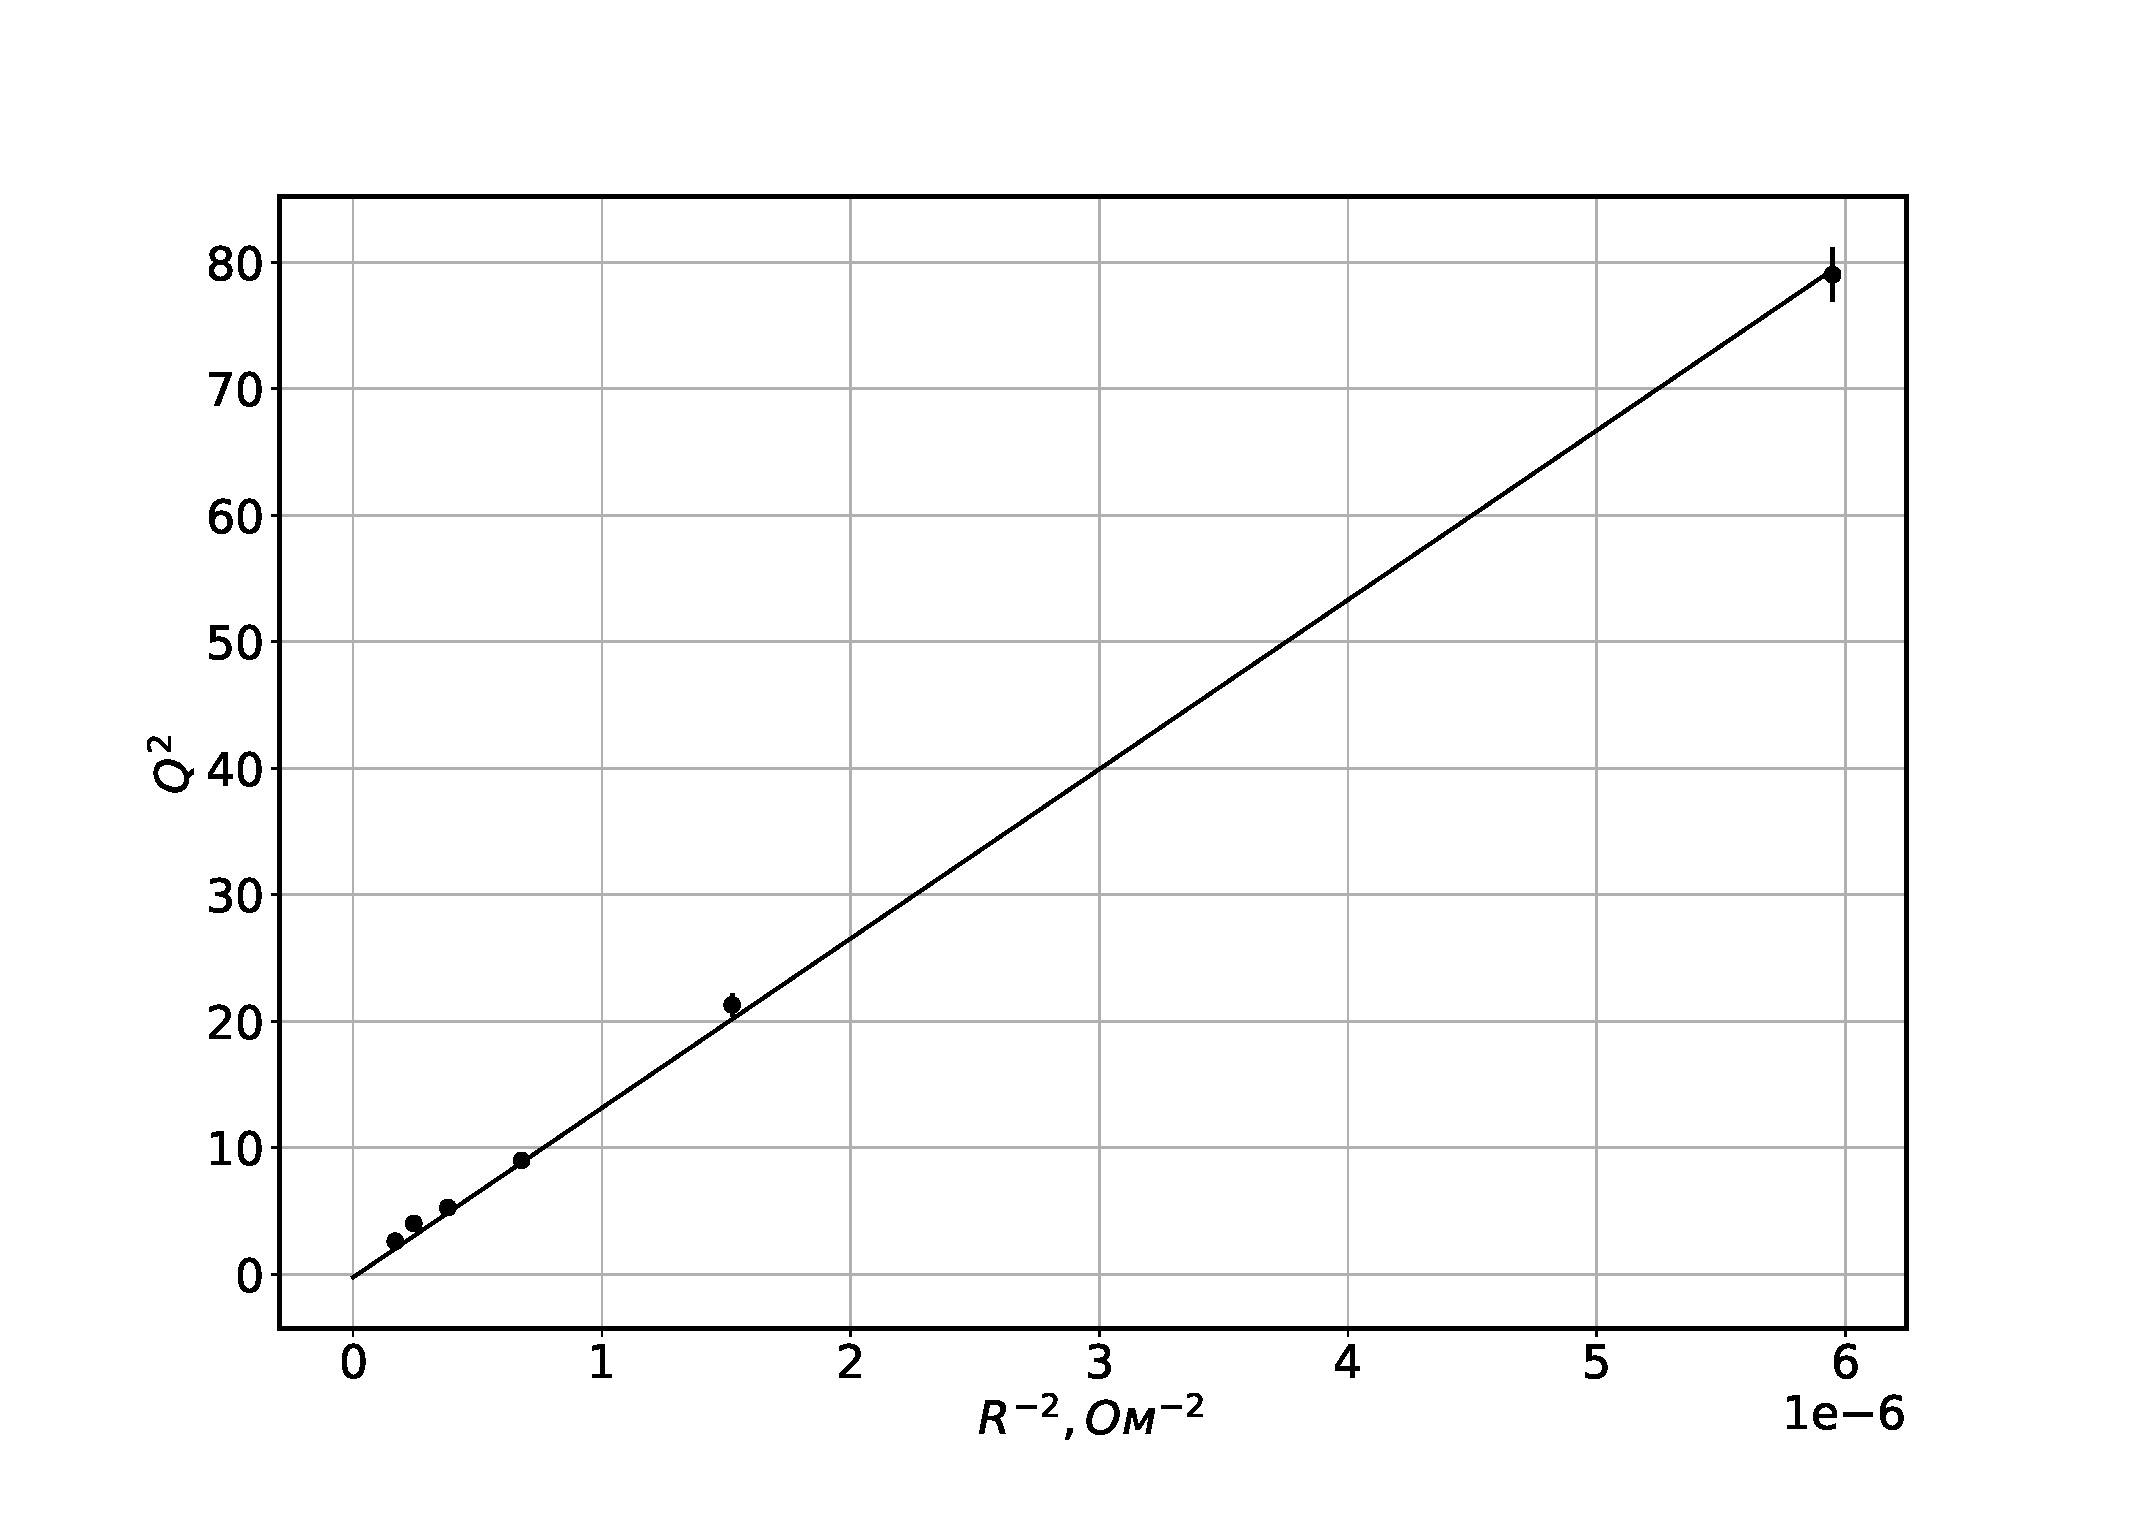
\includegraphics[width=0.7\textwidth]{RQ.eps}
	\caption{График линеаризованной зависимости добротности контура $Q^2$ от сопротивления контура $R^{-2}$.}
	\label{fig:RQ}
\end{figure}

Исследован процесс установления колебаний в конутре. Уствновлено, что при частоте источника, близкой к собственной 
частоте контура амплитуда колебаний монотонно возрастает (Рис. \ref{pic:1}). В то время как при частотах, 
далёких от собственной наблюдаются биения (Рис. \ref{pic:2}). Такое же поведение предсказывалось и теорией.
\begin{figure}[H]
	\centering
	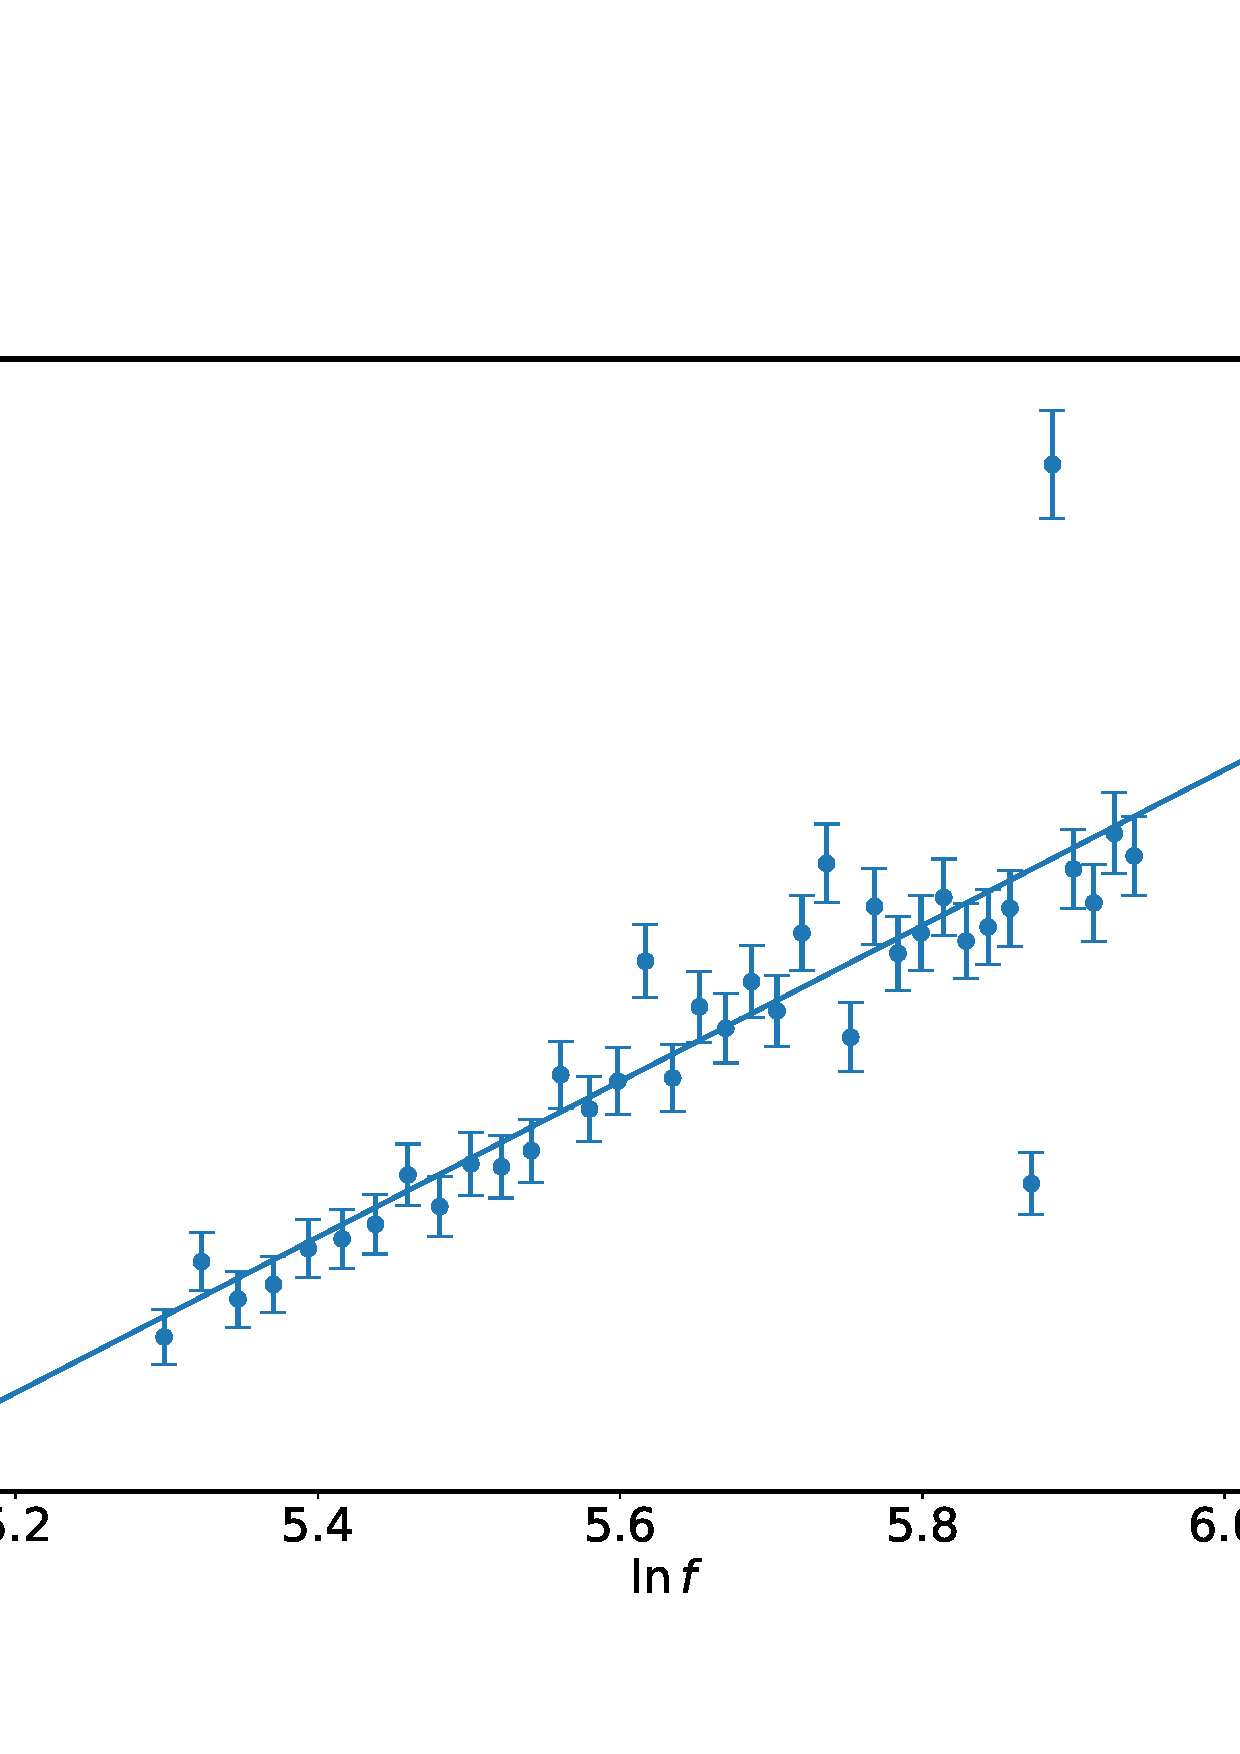
\includegraphics[width=0.6\textwidth]{3.jpg}
	\caption{График установления колебаний при частоте источника, близкой к собственной частоте контура.}
	\label{pic:1}
\end{figure}
\begin{figure}[H]
	\centering
	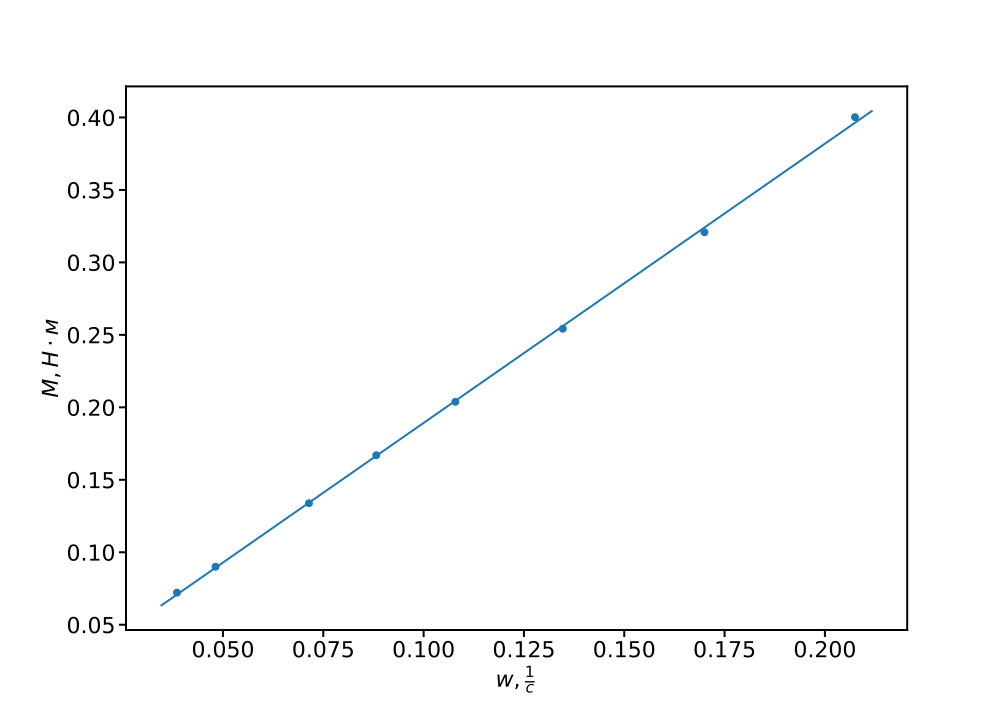
\includegraphics[width=0.6\textwidth]{2.jpg}
	\caption{График установления колебаний при частоте источника, далёкой от собственной частоты контура.}
	\label{pic:2}
\end{figure}

\section*{Выводы}
Измерена зависимость свободных колебаний контура в зависимоти от его ёмкости. Полученная зависимость полностью 
совпала с теоретически предсказанной. Получена зависимость добротности контура от его сопротивления. Несколькими 
способами определено критическое сопротивление контура. Рассмотрен процесс установления колебаний в контуре при 
различных частотах. Установлено, что при частотах, близких к собственной частоте контура наблюдается монотонно-возрастающая 
зависимоть амплитуды колебаний от частоты, тогда как при частотах источника, сильно отличабщихся от собственной частоты, наблюдаются биения.

\section*{Использованная литература}
\begin{thebibliography}{9}
	\bibitem{LabBook}
	Лабораторный практикум по общей физике, Том 2, под редакцией А. Д. Гладуна
\end{thebibliography}
\end{document}